%%%%%%%%%%%%%%%%%%%%%%%%%%%%%%%%%%%%%%%%%
% University Assignment Title Page 
% LaTeX Template
% Version 1.0 (27/12/12)
%
% This template has been downloaded from:
% http://www.LaTeXTemplates.com
%
% Original author:
% WikiBooks (http://en.wikibooks.org/wiki/LaTeX/Title_Creation)
%
% License:
% CC BY-NC-SA 3.0 (http://creativecommons.org/licenses/by-nc-sa/3.0/)
% 
% Instructions for using this template:
% This title page is capable of being compiled as is. This is not useful for 
% including it in another document. To do this, you have two options: 
%
% 1) Copy/paste everything between \begin{document} and \end{document} 
% starting at \begin{titlepage} and paste this into another LaTeX file where you 
% want your title page.
% OR
% 2) Remove everything outside the \begin{titlepage} and \end{titlepage} and 
% move this file to the same directory as the LaTeX file you wish to add it to. 
% Then add \input{./title_page_1.tex} to your LaTeX file where you want your
% title page.
%
%%%%%%%%%%%%%%%%%%%%%%%%%%%%%%%%%%%%%%%%%
%\title{Title page with logo}
%----------------------------------------------------------------------------------------
%	PACKAGES AND OTHER DOCUMENT CONFIGURATIONS
%----------------------------------------------------------------------------------------

\documentclass[12pt]{article}
\usepackage[english]{babel}
\usepackage[utf8x]{inputenc}
\usepackage{amsmath}
\usepackage{graphicx}
\usepackage[colorinlistoftodos]{todonotes}
\usepackage{listings}
\usepackage{color}
\usepackage{url}
\usepackage{booktabs}
\usepackage{hyperref}

\definecolor{codegreen}{rgb}{0,0.6,0}
\definecolor{codegray}{rgb}{0.5,0.5,0.5}
\definecolor{codepurple}{rgb}{0.58,0,0.82}
\definecolor{backcolour}{rgb}{0.95,0.95,0.92}
 
\lstdefinestyle{mystyle}{
    backgroundcolor=\color{backcolour},   
    commentstyle=\color{codegreen},
    keywordstyle=\color{magenta},
    numberstyle=\tiny\color{codegray},
    stringstyle=\color{codepurple},
    basicstyle=\footnotesize,
    breakatwhitespace=false,         
    breaklines=true,                 
    captionpos=b,                    
    keepspaces=true,                 
    numbers=left,                    
    numbersep=5pt,                  
    showspaces=false,                
    showstringspaces=false,
    showtabs=false,                  
    tabsize=2
}

\lstset{style=mystyle}

\textheight=250truemm \textwidth=160truemm 
\hoffset=-10truemm \voffset=-20truemm

\begin{document}

\begin{titlepage}

\newcommand{\HRule}{\rule{\linewidth}{0.5mm}} % Defines a new command for the horizontal lines, change thickness here

\center % Center everything on the page
 
%----------------------------------------------------------------------------------------
%	HEADING SECTIONS
%----------------------------------------------------------------------------------------

\textsc{\LARGE Ukrainian Catholic University}\\[1cm] % Name of your university/college
\textsc{\Large  Faculty of Applied Sciences}\\[0.5cm] % Major heading such as course name
\textsc{\large Data Science Master Programme}\\[0.5cm] % Minor heading such as course title

%----------------------------------------------------------------------------------------
%	TITLE SECTION
%----------------------------------------------------------------------------------------
\vspace*{1cm}

\HRule \\[0.4cm]
{\Large \bfseries Comparing of FACT properties of baseline and top models for prediction of household poverty level in  Costa Rica}\\[10pt]
{\large \bfseries Responsible Data Science final project report}\\[0.4cm] % Title of your document
\HRule \\[1cm]
 
%----------------------------------------------------------------------------------------
%	AUTHOR SECTION
%----------------------------------------------------------------------------------------
\vspace*{1cm}
 
% If you don't want a supervisor, uncomment the two lines below and remove the section above
\Large \emph{Authors:}\\
Maksym \textsc{Gontar}\\
Mikhail \textsc{Lebedev}\\
Oleh \textsc{Lukianykhin}\\
Roman \textsc{Moiseiev}\\[1cm] % Your name

%----------------------------------------------------------------------------------------
%	DATE SECTION
%----------------------------------------------------------------------------------------
\vspace*{1cm}
{\large 12 May 2019}\\[2cm] % Date, change the \today to a set date if you want to be precise

%----------------------------------------------------------------------------------------
%	LOGO SECTION
%----------------------------------------------------------------------------------------


\includegraphics[height=5cm]{images/UCU-Apps.png}\\[1cm] % Include a department/university logo - this will require the graphicx package
 
%----------------------------------------------------------------------------------------

\vfill % Fill the rest of the page with whitespace

\end{titlepage}

\begin{abstract} % 1 par [RM]
    This project is dedicated to the comparison of models of different complexity in the context of fairness and transparency. Prediction of the family’s poverty level in Costa Rica was chosen as the use case for consideration. The corresponding Kaggle competition resulted in several baseline models as well as top performing ones. In this work baseline and sophisticated solutions are investigated from the point of view of responsible data science. This creates a precedent of model selection and tuning based not only on quality metrics but meta-conditions, caused by developers responsibility. Also, the application of existing tools, in particular, SHAP, to ease decision making for both types of models is discussed. Results and conclusions of the investigation are described in this report.
\end{abstract}

\section{Introduction}~~~ 
    Currently, the main focus of Data Science and Machine Learning research lays into the field of efficiency. General approaches, algorithms and specific tools are developed to produce results of the best quality according to the formally defined quality metrics while utilizing a reasonable amount of resources. In particular, space and performance requirements, prediction quality and clever use of an available training data are considered. Interpretability, transparency, fairness and other aspects of responsible development are trending, but still not widely practiced.

    At the same time, the best models for many applied tasks are sophisticated. Intuitively and practically this leads to complicated interpretability. Moreover, models efficient on the available data are doing their best in reproducing biases present in the data. Thus the question of widening quality requirements for DS projects should be raised.

\section{Motivation}~~~
    First applications of Machine Learning were pretty technically oriented and applied to simple, practical problems. These attempts were successful, in particular, because subject field constraints were technical as well; there were no specific regulations or requirements from the ethical point of view. Thus, previous results are mostly not touching the ethical aspects of the development.
    
    However, impressive results of these applications lead to continually increasing business value, as well as growing trust to such solutions. Because of that, to stay competitive, companies of any kind are trying to make use of Data Science and Machine Learning. Consequently, applications in human-related fields appear, e.g. healthcare, insurance, social services etc. In this fields transparency, accuracy, fairness and confidentiality are of much higher importance.
    
    Hence, bringing these aspects into a spotlight of model tuning and selection will result in a better development process. It will be more consistent and reliable, as well as solutions will be. As a typical Data Science project development process goes from a simple baseline solution to a sophisticated one, it is important to understand how a solution changes during the mentioned transformation from the point of view of responsible development.
    
    Providing insights on Data Science project development that can ease an application of responsible development aspects in future projects is expected to be the impact of this report.

\section{Problem Formulation}~~~
    As it was discussed earlier, the main focus of this work is to analyze and compare the baseline solution with top performing one for a specific use case from the point of view of responsible development. In particular, how biases in the data are consumed, how fair predictions are and how flaws can be fixed.

    To this end, certain use case should be considered. The socially significant problem should be chosen, such that fairness and transparency of a solution are of crucial importance for the real-world applicability. This way results of the work can bring practical benefits, but not only be toy example for educational purposes.

    Thus, the prediction of the households poverty level in Costa Rica was chosen. This problem was released to the Kaggle community by The Inter-American Development Bank \cite{kaggle}, the largest source of development financing for Latin America and the Caribbean. Traditional instruments of determining financial need don’t work well when considering the poorest segment of the population, as limited data about their income and expense is available. Thus, organizations that make use of such a classification use Proxy Means Test as a best practice. It is a prediction based on the family’s observable household attributes. 
    
    The formulated problem was to determine the level of financial vulnerability for the household, based on the data about its’ members. The extensive dataset was provided with 140 features and ca. 29 000 entries, with four possible values of the target variable - a poverty of the household -  Extreme, Moderate, Vulnerable, Non-Vulnerable. The target quality metric was macro F1-score, i.e. an arithmetic average of F1-scores for each of the four possible classes. 
    
    Solving this problem with modern methods can improve current classification results and consequently have a positive influence on many lives in Costa Rica. Moreover, common problems are appearing all the time in social, public and community services all around the globe, as resources are limited, and one should make sure that right people receive an appropriate amount of aid. So, the solution can be used in other cases.
    
    As no cases of comparison of baseline and top performing models for the same Machine Learning task were found, the Related Work section is skipped. Details on tools and approaches applied can be found in the Approach to solution section.
    
\section{Approach to solution}
% some text required here?
\subsection{Use case analysis}~~~
    Among the many results created by the Kaggle community to solve this problem, the most outstanding one was released by Will Koehrsen \cite{kaggle_2}. It is a well-structured, clear and concise description of the solution development process. What is even more important it reflects all steps of the development of the Data Science solution according to the CRISP methodology: problem understanding, data understanding, data preparation, solution development and evaluation, iteration over previous steps to reach the desired performance. I.e. it provides extensive data analysis with cleaning and feature engineering steps, baseline model and stepwise improvements until the top-performing one. On the other side, focus in the model selection, and tuning was totally on the target quality metric. Taking into account all the facts above it was chosen as an ideal fit for the purpose of our analysis.
    
\subsection{SHAP}~~~
    To investigate results of model development and application one can investigate feature importance; influence of particular feature values and their combinations on prediction for a particular data point; changes in model behaviour and prediction caused by changes in the data consumed. As topic of model interpretability and fairness is in the spotlight last years, several efficient tools were created for these purposes. However, SHAP \cite{NIPS2017_7062} library was utilized in this work as this new tool has become a swiss knife for machine learning model analysis from the point of view of responsible development.
    
\section{Results}~~~

    Baseline model is Random Forest, top performing one is XGBoost. Exact values of parameters can be found in the source code. %[TBD]
    For the following experiments model with the parameters for baseline and best case were taken and trained on the subsample of the labelled data. Confusion matrix was built for predictions for the remaining labelled data. Train part is 75\% of the labelled data. The following confusion matrix was received for the baseline model:
    \begin{center}
        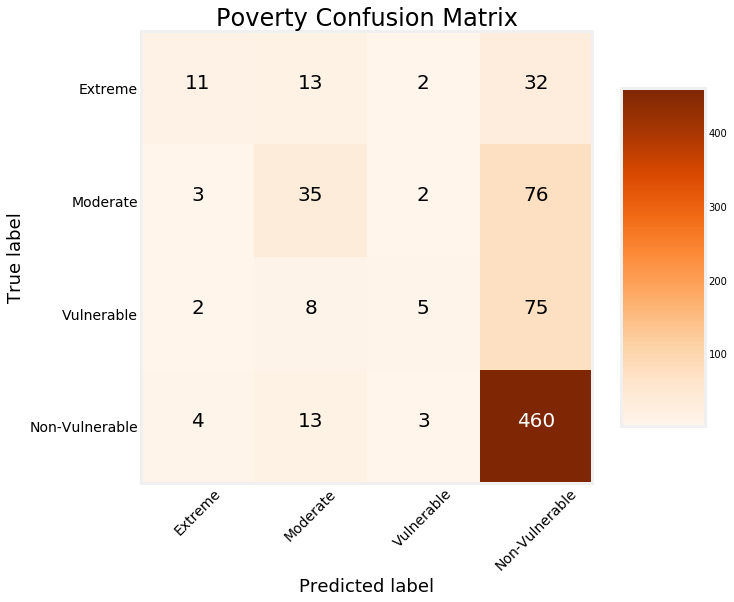
\includegraphics[width=\textwidth]{images/confusion_matrix_rf.png}
    \end{center}

    The bias of the model is observed - it tends to classify households as non-vulnerable. Most likely, as classes are unbalanced in the data.
    The following confusion matrix was received for the top model:
    \begin{center}
        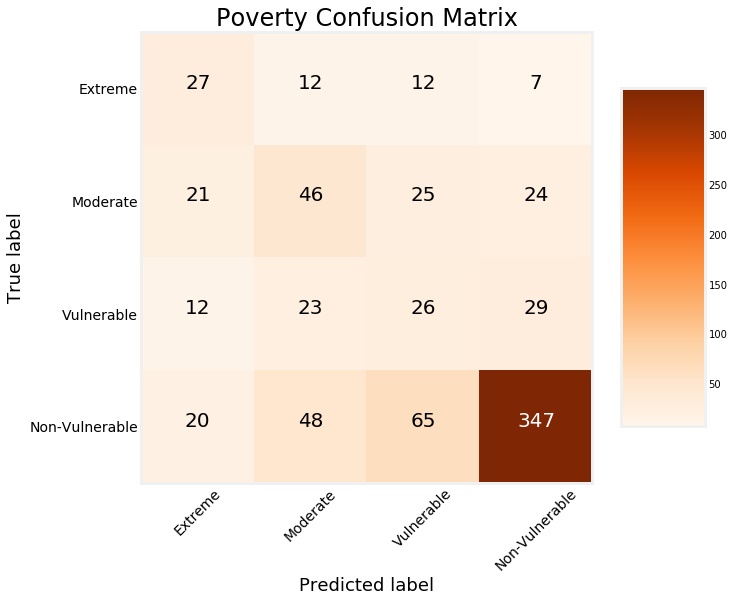
\includegraphics[width=\textwidth]{images/confusion_matrix_lgbm.png}
    \end{center}


    In this case, the reversed shift is observed. The model tends to classify fewer entries as non-vulnerable. However, there is a significant increase in erroneously classified objects of the Non-Vulnerable class. Taking into account the original problem this can be even worse, as leads to inefficient distribution of funds, while still not protecting a significant part of poor citizens.
    
    On the other side, the baseline model is good enough in identifying households of classes other than Non--Vulnerable. So with human supervision on cases, where prediction is Non-Vulnerable, such a system could work and reduce the workload on social government workers.
    
    Thus, we see that simpler models can be superior to better-performing ones considering an application and ethical aspects. Let’s investigate where and why models are making mistakes.
    
    \subsection{Non-vulnerable vs Extreme}
    \subsubsection{Baseline Model}~~~
        4 Non-Vulnerable households were classified as Extremely vulnerable. 32 Extremely vulnerable households were classified as Non-Vulnerable. To find the reasoning behind such prediction we have investigated these cases using SHAP.
        
        Overall most important features for the model are dependency, group of education-related features and group of property related features.
        
        For 4 Non-Vulnerable households that were classified as Extreme vulnerable - that was households with the low level of education, the existence of the dependent peoples and issues with walls/roof/floor, absence of electricity, toilet, etc. And even for the human, it's hard to distinguish proper class.
        
        For 32 Extreme vulnerable households that were classified as Non-Vulnerable - the main reason is an imbalance in the data, which leads to the higher base value that the model predicts. 
        
        Following insights were found for the Baseline model:
        \begin{itemize}
            \item Highly educated peoples that have bad signs in property related features are not marked as extremely vulnerable because of the dominance of education-related features
            \item If people with extreme poverty don't have substantial issues with the property, they will be marked as Non-Vulnerable
            \item If people with extreme poverty have at least some items related to prosperity (TV, phones, etc.), then with high probability they will be marked as non-vulnerable
            \item People with a low level of education may be misclassified as extremely vulnerable if they have issues with the property
        \end{itemize}
        
    \subsubsection{Top Model}~~~
        20 Non-Vulnerable households were classified as Extremely vulnerable. 7 Extremely vulnerable households were classified as Non-Vulnerable, which is fairer than the baseline model.

        Set of the most important features is similar, but different engineered features have more weight for example edjefe - years of education of a male head of household. After an investigation of data using SHAP, we may see that the reasons behind misclassification are similar to that in the Baseline model. Although more specific features are used to describe an education, state of property and issues. From a human perspective, it's even more complicated to get through.
        
        Following insights were found for the Baseline model:
        \begin{itemize}
            \item More specific features important for the model
            \item Model is more confident in its predictions
        \end{itemize}
        
    \subsection{Non-vulnerable vs Moderate}
    \subsubsection{Baseline Model}~~~
        13 Non-Vulnerable households were classified as Moderate poor. 67 Moderate poor households were classified as Non-Vulnerable. All 13 observations from the first category and 20 randomly sampled observations from the second category were analyzed using SHAP library plots. The experiment was done to find the minimal changes in the most influential features for the positive change in the prediction.

        Insights for the false Moderate:
        \begin{itemize}
            \item The features, which contributes most to the misclassification in the case of false Moderate are a high dependency, low escolari-min, low meaneduc, walls+roof+floor, low phone-per-capita, low escolari-max, high eviv1, high warning, low rooms-per-capita, low floor, high escolari/age-min, low instlevel8-max. 
            \item Observations \# 4, 11, 12 from the sample had a higher chance to be classified as false Extreme poor rather than true Non-Vulnerable. 
            \item 25\% of the sample predictions could be corrected by 20\% increase of escolari-max (Maximum years of schooling of the household members). 
            \item In case of observation \# 5 the increase of escolari-max starting from 40\% causes the even worse misclassification as false Extreme poor - which seems to be the example of biased ML application
        \end{itemize}
        
        Insights for the false Non-Vulnerable:
        \begin{itemize}
            \item False Non-vulnerable predictions in the case are explained by low dependency, high phones-per-capita, high escolari-min, hight meaneduc, high instlevel8-max, low warning, high walls+roof+floor, high escolari-max, high instlevel8-sum, high escolari-sum, high cielorazo, high escolari/age-min, high inst-max, low intslevel2-sum.
            \item 14\% of the sample predictions could be corrected by 60\% decrease of phones-per-capita (Number of mobile phones per household members). 
            \item 9\% of the sample predictions could be corrected by 70\% increase of dependency (number of members of the household younger than 19 or older than 64 divided by the number of member of household between 19 and 64). 
        \end{itemize}
        
    \subsubsection{Top Model}~~~
        51 Non-Vulnerable households were classified as Moderate poor. 22 Moderate poor households were classified as Non-Vulnerable. 5 randomly sampled observations from both categories were analyzed using SHAP library plots. The experiment was done to find the minimal changes in the most influential features for the positive change in the prediction.
        
        Insights for the false Moderate:
        \begin{itemize}
            \item False Moderate prediction in the case is explained by low walls+roof+floor, high dependency, high age-sum, low escolari-min, high escolari/age-max, low floor, low rooms-per-capita, low phones-per-capita.
            \item 25\% of the sample predictions could be corrected by 20\% increase of escolari/age-sum (years of schooling divided by sum of age of household members). 
            \item 25\% of the sample predictions could be corrected by 70\% decrease of dependency (number of members of the household younger than 19 or older than 64 divided by the number of member of household between 19 and 64). 

        \end{itemize}
        Insights for the false Non-Vulnerable:
        \begin{itemize}
            \item False Non-vulnerable predictions in the case are explained by high phones-per-capita, high rent-per-capita, high v2a1, high escolari-min, high walls+roof+floor, low dependency, low escolari/age-min, high bonus, hight meaneduc, high edjefe.
            \item Two obs. with extreme high influence of high escolari-max feature, and one obs. with extreme high influence of rent-per-capita feature.
            \item 33\% of the sample predictions could be corrected by 40\% decrease of phones-per-capita (years of schooling divided by sum of age of household members). 
        \end{itemize}
        
    \subsection{Non-vulnerable vs Vulnerable}
    \subsubsection{Baseline Model}~~~
    
    3 Non-Vulnerable households were classified as Vulnerable. 75 Vulnerable households were classified as Non-Vulnerable.
    To take a closer look at these misclassified cases household data and prediction for it were investigated with the help of SHAP library. All 3 samples from the first category and 5 randomly drawn samples from the second one were taken for consideration.
    The following insights were found:
        \begin{itemize}
            \item Misclassified cases are edge cases. Even for a human, it is hard to classify these cases.
            \item Features related to education are important. Their influence can be both strongly negative or strongly positive for the probability of certain class. Seems like, the model might overfit for certain values of these features, as in some cases influence on prediction is exactly opposite to the expected for a proper label of the entry.
            \item Difference between predicted probabilities is tiny, 1-3\% for many cases. In simple words, this means that the model is not sure about prediction.
        \end{itemize}    

    \subsubsection{Top Model}~~~

    68 Non-Vulnerable households were classified as Vulnerable. 29 Vulnerable households were classified as Non-Vulnerable.
    To take a closer look at these misclassified cases household data and prediction for it were investigated with the help of SHAP library. 5 randomly drawn samples were from both categories for consideration.
    These are insights found:
        \begin{itemize}
            \item Features related to education are important. However, their influence changes from case to case can be both strongly negative or strongly positive for the probability of certain class.
            \item Difference between predicted probabilities is big. So, model misclassified households with much more confidence.
            \item Features created during feature engineering steps are of strong importance and working properly, as they are decreasing the predicted probability for some classes while increasing it for others
        \end{itemize}
        
        Comparison of both models leads to the following insights:
        \begin{itemize}
            \item SHAP utilization helps to understand why certain predictions were made and ease decision making for a human supervisor.
            \item Overfitting negatively influence both prediction quality and how the model can be used as a supportive tool for decision making.
            \item Seeing the predicted probabilities of classes (or proxy score for XGBoost) is extremely useful for the understanding of model nature and overfitting level.
            \item Overfitting negatively influence both prediction quality and how the model can be used as a supportive tool for decision making.
            \item Some features have very strong influence: features related to the education of household members; features created during feature engineering stage - aggregating signs of poor/prosper household. These features require more attention during model development and analysis of results.
        \end{itemize}
        
\section{Conclusions and Future work}~~~
    All source code can be found at our GitHub repository \cite{our_github}. Results of this work satisfied our research interests reflected in the aim of the project, as following insights were found:
    \begin{enumerate}
        \item Fighting overfitting is very important when a model is expected to be used as a supportive tool in decision making. A simpler model can be more useful for such purpose.
        \item Balancing classes in the training data is a must, not only for higher prediction quality but for fairness and interpretability of results.
        \item Making decision based on such a big number of features is hard. The supportive tool can be very beneficial. 
        \item Expert based feature engineering and automated solutions for it can strongly help in solving real-life problems, even though for a supportive tool explainable features made by a human expert are much easier to utilize.
    \end{enumerate}
    
    However, there are the following options for improvements and further work:
    \begin{enumerate}
        \item Generalize approach of comparison baseline and sophisticated models
        \item Create common guidelines for responsible development taking into account fairness and accuracy.
    \end{enumerate}

\bibliographystyle{unsrt} %Used BibTeX style is unsrt
\bibliography{references}

\end{document}
